\documentclass[a4paper,11pt]{article}
%\usepackage{pst-eucl}
%\usepackage[applemac]{inputenc}
\usepackage[english]{babel}
\usepackage[T1]{fontenc}
\usepackage{graphicx}
\usepackage{xcolor}
\usepackage{amssymb}
\usepackage{amsmath}
\usepackage[utf8]{inputenc}
\usepackage{mathtext}
\usepackage{algorithm,algorithmic}
\usepackage{setspace}
\usepackage{textcomp}
\usepackage{geometry}
\geometry{hmargin=2cm,vmargin=2cm}
\usepackage{lscape}
\renewcommand{\baselinestretch}{1.2}
\usepackage{cite}
\usepackage{natbib}

%opening

\title{Physical Oceanography, MO7015}
\author{Problems and exercises (2016)}

\begin{document}
\date{}
\maketitle

\section{Wind driven circulation and potential vorticity (Kristofer Doos)}
\begin{enumerate}
\item Potential vorticity is defined as following:
\begin{equation}
P=\frac{\varsigma+f}{h} 
\end{equation}
Where $\varsigma$ is the relative vorticity $\frac{\partial v}{\partial x} - \frac{\partial u}{\partial y}$ and $f$ the coriolis parameter. Derive an expression for potential vorticity if a wind stress $\tau^{w} = [\tau^{x},\tau^{y}]$ and a Rayleigh friction [$\Gamma u,\Gamma v]$ is added to the nonlinear shallow water equations:
\begin{equation}
\frac{\partial u}{\partial t} + u\frac{\partial u}{\partial x} + v\frac{\partial u}{\partial y}-fv = -g\frac{\partial \eta}{\partial x}
\end{equation}
\begin{equation}
\frac{\partial v}{\partial t} + u\frac{\partial v}{\partial x} + v\frac{\partial v}{\partial y}+fu = -g\frac{\partial \eta}{\partial y}
\end{equation}
\begin{equation}
\frac{Dh}{Dt} = -h\left(\frac{\partial u}{\partial x} + \frac{\partial v}{\partial y}\right)
\end{equation}
where $\eta$ the free surface and $h$ the water depth (with varying bathymetry).

\item Does the flow described by the expression derived in (1) follow f/H contours?
Why? Why not?\\
Identify areas in the ocean where the flow is likely to follow f/H contours.

\item Assume that the Rossby number $U/(fL) << 1$ and that $\eta/H << 1$ and linearize the expression derived in exercise (1) (You will get something that looks like the Stommel solution).

\item Write the expression derived in (4) on a stream function form, where
\begin{equation}
\frac{\partial \psi}{\partial x} = v, \frac{\partial \psi}{\partial y} = -u
\end{equation}
\end{enumerate}

\section{Sverdrup Circulation (Exam 2012-08-30)}
Consider the quasi-geostrophic equations :
\begin{equation}
-fv = -g\frac{\partial \phi}{\partial x} + \frac{\partial \tau^{x}}{\partial z},
\end{equation}
\begin{equation}
fu = -g\frac{\partial \phi}{\partial y} + \frac{\partial \tau^{y}}{\partial z},
\end{equation}
\begin{equation}
\frac{\partial \phi}{\partial z} = b,
\end{equation}
\begin{equation}
\frac{\partial u}{\partial x} + \frac{\partial v}{\partial y} + \frac{\partial w}{\partial z} = 0,
\end{equation}
where $f = f(y)$ (and $\beta = df/dy$).
\begin{enumerate}
\item Derive the Sverdrup relation for the depth-integrated vertical transport, that is  $\int_{-H}^{0} v \, \mathrm{d}z$, where $H$ is the depth of the ocean. \textit{State the assumptions you make to obtain the Sverdrup relation.}
\item Define a transport stream function $\psi$ such that
\begin{equation}
\left(\int_{-H}^{0} u \, \mathrm{d}z,\int_{-H}^{0} v \, \mathrm{d}z\right) = \left(-\frac{\partial \psi}{\partial y}, \frac{\partial \psi}{\partial x}\right).
\end{equation}
Assume a wind field given by $\tau^{x}(y) = \tau_{0} \text{sin}(\frac{\pi y}{2L})$ and use the Sverdrup relation to calculate $\psi$; assume that there are coasts at x = 0 and x = B.
\item Sketch $\psi$ between $y = -L$ and $y = L$. Sketch also qualitatively the boundary layer near the coast.
\item What additional physics has to be included in the Sverdrup relation [in Eqs. (6,7)] to obtain a boundary layer that can satisfy the condition of zero normal flow at the boundaries?
\end{enumerate}


\section{Coastal jet (Exam 2012-08-30)}
Consider an infinite long coast line, parallel to the y axis, located at $x = 0$, with an ocean of a constant depth $H$ located to the right ($x > 0$). At time $t = 0$ a wind starts blowing that is associated with a constant wind stress in the y direction ($\tau_{y}$). The flow that results is independent of the y coordinate. Assume further that the flow along the coast is in geostrophic balance and use the shallow water equations to determine the flow field $[u(x, t),v(x, t),\eta(x, t)]$:
\begin{equation}
-fv = -g\frac{\partial \eta}{\partial x},
\end{equation}
\begin{equation}
\frac{\partial v}{\partial t} + fu = \frac{\tau_{y}}{H},
\end{equation}
\begin{equation}
\frac{\partial \eta}{\partial t} = -H\frac{\partial u}{\partial x}.
\end{equation}
The initial conditions at time $t = 0$ are $\eta = 0$ and $v = 0$. At the coast ($x = 0$), the boundary condition $u = 0$ applies.

\section{Kelvin Waves (Exam 2012-08-30)}
Consider the shallow water equations :
\begin{equation}
\frac{\partial u}{\partial t}-fv = -g\frac{\partial \eta}{\partial x}
\end{equation}
\begin{equation}
\frac{\partial v}{\partial t}+fu = -g\frac{\partial \eta}{\partial y}
\end{equation}
\begin{equation}
\frac{\partial \eta}{\partial t} = -H\left(\frac{\partial u}{\partial x} + \frac{\partial v}{\partial y}\right)
\end{equation}
\begin{enumerate}
\item Derive the solution describing coastal Kelvin waves that propagate along a coast line that is parallel to the x-axis. Treat the Coriolis parameter f as a constant. State clearly the phase speed and the propagation direction of the Kelvin wave.
\item Sketch how costal and equatorial Kelvin wave propagate from point A to B in Fig. 1. Sketch also the propagation direction of costal Kelvin waves around Antarctica.
\end{enumerate}
\begin{figure}[t]
\center
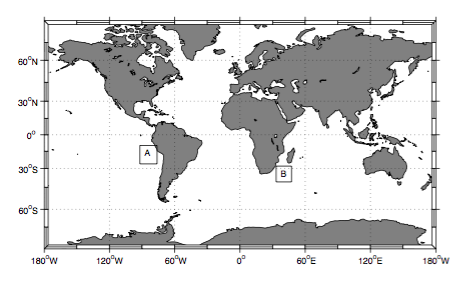
\includegraphics[width=30pc,angle=0]{Fig1}
\caption{}
\end{figure}

\section{Waves (Peter Lundberg)} 
\begin{enumerate}
\item Assuming that $\eta = acos(kx - \omega t)$ and that $\frac{\partial u}{\partial x} + \frac{\partial w}{\partial z}  = 0$, derive the expression
$$
\Phi(x, z, t) = \frac{a\omega}{k} \frac{\text{cosh}(k(z + H))}{\text{sinh}(kH)} sin(kx - \omega t)
$$
for the velocity potential.
\item Derive an expression for the vertical Stoke's drift.\\
Hint : $u(x,z,t) = a\omega e^{kz} \text{cos}(kx - \omega t)$ and $w(x,z,t) = a\omega e^{kz} \text{sin}(kx - \omega t)$.
\end{enumerate}

\section{Internal waves (Jonas Nycander)} 
\begin{enumerate}
\item Derive the dispersion relation for internal waves from the hydrostatic primitive equations including the Coriolis term.
\item Starting from the general dispersion relation for internal waves, derive the expressions for the horizontal phase velocity and group velocity for the lowest vertical mode ($n = 1$) of hydrostatic, non rotating internal waves, whose frequency satisfies $f^{2} << \omega^{2} << N^{2}$. 
Estimate the horizontal group velocity numerically, assuming that $N = 10^{-2} \text{s}^{-2}$, and that the characteristic vertical scale of this mode is the thermocline depth, $H = 10^{3}$m.
\end{enumerate}

\section{Various wave problems (Johan Nilsson)} 
\begin{enumerate}

\item On decent day for surfing in the Baltic the surface waves have periods of about seven seconds. Use the dispersion relation for gravity waves in deep water
\begin{equation}
\omega = (g |k|)^{1/2},
\end{equation}
to calculate the wave length. How long does it take such waves to travel from around Gotland to Toro (surf spot near Nynashamn)?

\item You stand at a beach and surface gravity waves from a distant storm (located at a distance L) start to arrive. First the waves with long wave-lengths and wave-periods arrive as they travel fastest. Calculate how the frequency of the arriving waves change with time. Shows that the frequency of the arriving waves increases linearly with time. (Why does this rate decrease with the distance to the storm?) This can in principle be used to estimate the distance to storm at sea.

\item Consider non-rotating internal waves governed by the equations
\begin{equation}
\frac{\partial u}{\partial t} = -\frac{\partial \phi}{\partial x},
\end{equation}
\begin{equation}
\frac{\partial w}{\partial t} = -\frac{\partial \phi}{\partial z} + b,
\end{equation}
\begin{equation}
\frac{\partial u}{\partial x} + \frac{\partial w}{\partial z} = 0,
\end{equation}
\begin{equation}
\frac{\partial b}{\partial t} + wN^{2} = 0,
\end{equation}

Use the fact that the flow can be described by the stream function
\begin{equation}
(u,w) = \left(-\frac{\partial \psi}{\partial z}, \frac{\partial \psi}{\partial x} \right) 
\end{equation}
and derive the wave equation for $\psi$. Assume a plane wave on the form $\psi(x, z, t) = \psi_{0} \text{cos}(\omega t - kx - mz)$ and derive the dispersion relation. Sketch the flow (for $t = 0$) and indicate the velocity, buoyancy perturbation and the directions of the phase and group velocities.

\item Shallow-water Poincare waves are described by
\begin{equation}
\frac{\partial u}{\partial t}-fv = -g\frac{\partial \eta}{\partial x}
\end{equation}
\begin{equation}
\frac{\partial v}{\partial t}+fu = -g\frac{\partial \eta}{\partial y}
\end{equation}
\begin{equation}
\frac{\partial \eta}{\partial t} = -H\left(\frac{\partial u}{\partial x} + \frac{\partial v}{\partial y}\right)
\end{equation}
Derive and equation for $\eta$ and determine the dispersions relation for plane wave $\eta(x, y, t) = \eta_{0} \text{cos}(\omega t - kx - ly)$. Take l = 0 and sketch the phase and group velocities. Take again $l = 0$ and express $u$ and $v$ in terms of $\eta$; this is known as the polarization relations. 

\item (pure) Inertial oscillations can be described in complex notation as $\frac{\partial U}{\partial t} + ifU = X$, where $U = u+iv$ and $X = F_{x} +iF_{y}$ are the complex velocity and wind forcing vectors. Solve the velocity field resulting when a constant wind $X = iF_{y}$ is switched on at time $t = 0$. The ocean is at rest initially. Sketch the velocity and particle paths. A time integration gives the particle displacement.
\end{enumerate}

\section{Spin-up of the Sverdrup Circulation (Johan Nilsson)}
Consider the following thought experiment. Assume that the ocean is at rest and the winds are suddenly switched on. Focus on the Atlantic subtropics and describe how the Sverdrup Circulation becomes established (discuss the role of Rossby waves). If the zonal width of the basin is $L$, how long time does it take to establish the Sverdrup Circulation in the basin? (Answer: $L/(\beta a^{2})$)

\section{Thermohaline circulation (Exam 2015-01-16)}
Consider a Stommel box model specified by the following equation
\begin{equation}
V \frac{d\Delta S}{dt} = -\Delta S M + S_{0}F,
\end{equation}
where $\Delta S$ is the salinity difference between the boxes, $M$ the flow, $S_{0} = 35$ constant reference salinity, $V$ the volume and $F$ the freshwater supply. The flow is specified by
\begin{equation}
M=k|\Delta \rho_{T} -\beta \Delta S|,
\end{equation}
 where $\Delta \rho_{T}$ is the density difference associated with the temperature difference and $\beta$ the haline expansion coefficient, and k a constant.

\begin{enumerate}
\item Describe the two types of steady states that can exist in Stommel's box model. Explain briefly the physics that allows for the two different states.

\item Consider Eq. 8 and find the $\Delta S$ values that correspond to steady states. Discuss briefly the properties of the solutions and show that no thermally-dominated states exists when $\frac{\beta S_{A}F}{k\Delta \rho_{T}^{2}} > 1/4$. Sketch also how the steady-state values of $\Delta S$ and $M$ depend on $F$.

\item Determine the stability of the steady-state solutions above, and calculate the maximun value of $\Delta S$ for which the thermally-dominated solution is stable.

\item Illustrate qualitatively the salinity distribution (in the vertical-latitudinal plane) in the Atlantic and Pacific Oceans. Comment briefly on how Stommel's box could be used in an attempt to explain the salinity distribution difference between the North Pacific and North Atlantic.
\end{enumerate}


\end{document}